% =====================================================================================
%  MSGF-Net paper - compile on Overleaf (IEEEtran is built in) with pdfLaTeX + BibTeX.
%  Red [PENDING: ...] marks = details still to be filled in (e-mail addresses).
% =====================================================================================
\IfFileExists{IEEEtran.cls}{\documentclass[conference]{IEEEtran}}{%
  \documentclass[10pt,twocolumn]{article}\usepackage[margin=0.7in]{geometry}}
\usepackage{amsmath,amssymb}
\usepackage{graphicx}
\usepackage{booktabs}
\usepackage{multirow}
\usepackage{xcolor}
\usepackage{tikz}
\usetikzlibrary{positioning,arrows.meta,fit,calc}
\usepackage{cite}
\usepackage[hidelinks]{hyperref}

% ---- fallbacks so the file also compiles without IEEEtran.cls --------------------
\makeatletter
\providecommand{\IEEEauthorblockN}[1]{#1\\}
\providecommand{\IEEEauthorblockA}[1]{\small #1}
\@ifundefined{IEEEkeywords}{\newenvironment{IEEEkeywords}{\par\noindent\textbf{\textit{Index Terms}---}}{\par}}{}
\makeatother
\newcommand{\pending}[1]{\textcolor{red}{[PENDING: #1]}}
\newcommand{\figorbox}[2]{\IfFileExists{#1}{\includegraphics[width=#2]{#1}}{%
  \fbox{\parbox[c][0.16\textheight][c]{#2}{\centering\small missing: \texttt{\detokenize{#1}}}}}}

\begin{document}

\title{Calibrated, Uncertainty-Aware Pulmonary Nodule False-Positive Reduction with Multi-Window Scale-Gated 3D Fusion and Size Estimation}

\author{\IEEEauthorblockN{Abdullah Asim, Hussnain Khalid and Rabia Masood}
\IEEEauthorblockA{Department of Computer Sciences, Bahria University Lahore Campus, Lahore, Pakistan\\
abdullahasimnaawaz@gmail.com, hussnainkhalid421@gmail.com, rabiamasood.bulc@bahria.edu.pk}}

\maketitle

\begin{abstract}
False-positive reduction is the stage of a lung-screening computer-aided detection (CAD) system that decides which of hundreds of candidate locations per CT scan are real pulmonary nodules. Most recent work optimises accuracy on re-balanced 2D patch sets and outputs only a class label, which neither reflects screening performance nor tells the radiologist how much to trust a mark or how large the nodule is. We propose MSGF-Net, a compact (3.35\,M parameter) 3D network that encodes each candidate with three Hounsfield-unit windows, analyses a 32\,mm local view and a 48\,mm context view in two residual squeeze-excitation streams, and fuses them with a scale-gated fusion block in which context recalibrates local features and a learned per-channel gate mixes the two scales. A diameter-regression head is trained jointly through homoscedastic-uncertainty weighting, and inference combines 8-view test-time augmentation with Monte-Carlo dropout on the classification head, followed by Platt calibration fitted on a validation subset. On the held-out LUNA16 subset~9 (88 scans, 105 nodules, 75{,}924 candidates; patient-level split, model selected on subset~8) MSGF-Net reaches a competition performance metric (CPM) of 0.903 (95\% CI 0.843--0.956), with 97.1\% sensitivity at 4 and 98.1\% at 8 false positives per scan. It additionally estimates nodule diameter with a mean absolute error of 0.45\,mm ($r=0.996$), reduces the expected calibration error from 0.0123 to 0.0007, and its predictive uncertainty identifies its own errors with an AUROC of 0.971. Ablations show that these clinically useful outputs come without a measurable loss in detection accuracy. Trained with the identical protocol, MSGF-Net outperforms a 3D ResNet-18 ($p=0.034$) with one tenth of its parameters and matches a plain 3D CNN of similar size, indicating that much of the accuracy stems from the protocol rather than the architecture alone. Placed behind a training-free candidate finder whose candidates are ranked by Laplacian-of-Gaussian response times a Hessian blobness score, the complete pipeline reaches 92.4\% candidate recall and a CPM of 0.867 (95\% CI 0.800--0.923) from raw CT. Without retraining, at operating points fixed on LUNA16 validation, it detects on average 75.4\% (up to 90.7\%) of 6{,}163 nodules in the independent low-dose screening data of LUNA25. Federated averaging across four simulated hospitals that share only model weights raises CPM from 0.665 (one hospital alone) to 0.808, against 0.880 for pooled data. The system is deployed in a clinician workstation with slice-level risk display and Grad-CAM explanations and in a patient application with a guideline-grounded, tool-using assistant.
\end{abstract}

\begin{IEEEkeywords}
lung cancer screening, pulmonary nodule, false-positive reduction, LUNA16, uncertainty estimation, calibration, 3D CNN, computer-aided detection
\end{IEEEkeywords}

% =====================================================================================
\section{Introduction}
Low-dose CT screening reduces lung-cancer mortality by 20\% in high-risk individuals~\cite{nlst2011}, but every screening scan must be searched for small pulmonary nodules, a tedious task in which nodules are missed. CAD systems typically combine a sensitive candidate detector with a false-positive (FP) reduction classifier that rejects the many vessels, scars and pleural structures among the candidates. The LUNA16 challenge~\cite{setio2017luna16} standardised this task on 888 CT scans from LIDC-IDRI~\cite{armato2011lidc} and introduced the competition performance metric (CPM): the mean sensitivity at 1/8, 1/4, 1/2, 1, 2, 4 and 8 FPs per scan.

Two gaps motivate this work. First, a considerable part of the recent literature evaluates 2D CNNs on re-balanced, augmented patch sets and reports accuracy~\cite{naseer2022sensors,geetha2022efficientnet,lv2024mifnet}. With roughly 484 negative candidates per positive in LUNA16, patch accuracy says little about FPs per scan; some works also describe the LUNA16 nodule/non-nodule classes as ``benign/malignant'', although LUNA16 contains no malignancy labels. Second, even strong FP-reduction systems such as multilevel contextual 3D CNNs~\cite{dou2017multilevel} output a single score. A radiologist additionally needs to know the nodule \emph{size}, which drives Lung-RADS management~\cite{lungrads2022}, whether the probability can be taken at face value (\emph{calibration}), and when the model is unsure (\emph{uncertainty}).

\textbf{Contributions.}
(1) A scale-gated fusion (SGF) block in which a 48\,mm context descriptor recalibrates the channels of a 32\,mm local feature map and a learned per-channel gate mixes the two scales inside one network; the gate is interpretable and correlates with nodule size.
(2) Multi-window HU encoding and a jointly trained diameter head (homoscedastic-uncertainty weighting~\cite{kendall2018multitask}) that turn the classifier into a size-aware model.
(3) Efficient uncertainty-aware inference: 8-view test-time augmentation with Monte-Carlo dropout~\cite{gal2016dropout} applied only to the head (encoders run once per view), Platt calibration~\cite{platt1999} on a validation subset, and an uncertainty-based triage analysis.
(4) A rigorous protocol: patient-level official subsets, model selection on validation only, every candidate of the test subset scored, CPM with bootstrap confidence intervals and paired significance tests, including honestly reported negative results (hard-negative fine-tuning) and a same-protocol comparison with three standard 2.5D and 3D architectures.
(5) An end-to-end evaluation from raw CT with our own candidate finder, in which a robust field-of-view-aware lung mask and Hessian blobness ranking raise candidate recall from 53\% to 92\%, and an external validation on 6{,}163 nodules of the independent LUNA25 screening cohort~\cite{luna25}.
(6) A deployed system: clinician workstation (slice-level risk bar, Grad-CAM, image-based and clinical Brock risk) and patient web and Android app with a guideline-grounded, tool-using assistant.

% =====================================================================================
\section{Related Work}
\textbf{FP reduction on LUNA16.} The challenge paper~\cite{setio2017luna16} reports CPMs between 0.758 and 0.908 for the FP-reduction track; the best system, CUMedVis, used three 3D CNNs with different receptive fields whose output probabilities were averaged~\cite{dou2017multilevel}. MSGF-Net instead fuses scales at feature level inside one network with a learned gate.
\textbf{2D patch classifiers.} AlexNet/VGG/EfficientNet-type models applied to 2D crops~\cite{naseer2022sensors,geetha2022efficientnet} and multi-scale lightweight designs such as MIFNet~\cite{lv2024mifnet} report high accuracy on balanced patch sets, which is not comparable with CPM.
\textbf{Segmentation.} Transformer-U-Net hybrids, including federated variants~\cite{turjya2026federated}, address nodule delineation, a complementary task.
\textbf{Calibration and uncertainty.} Modern networks are over-confident~\cite{guo2017calibration}; MC dropout~\cite{gal2016dropout} and ensembles~\cite{lakshminarayanan2017ensembles} provide predictive uncertainty. These are rarely evaluated for nodule FP reduction, where the strong class imbalance and oversampling during training make raw probabilities especially miscalibrated.

% =====================================================================================
\section{Data and Protocol}
\textbf{LUNA16.} 888 CT scans (slice thickness $\le$2.5\,mm) with 1{,}186 nodules $\ge$3\,mm accepted by at least 3 of 4 radiologists (Table~\ref{tab:data}). We use the 754{,}975 candidates of \texttt{candidates\_V2} (1{,}557 positive). Findings in \texttt{annotations\_excluded} are neither TPs nor FPs, as in the official evaluation.

\begin{table}[t]
\centering
\caption{LUNA16 data used in this study.}
\label{tab:data}
\small
\begin{tabular}{@{}lr@{}}
\toprule
Scans (subsets 0--9) & 888 (89/88 per subset)\\
Scans with $\ge$1 nodule & 601\\
Reference nodules & 1{,}186\\
Diameter, mean $\pm$ SD (range) & 8.3 $\pm$ 4.8 (3.3--32.3) mm\\
Candidates (positive) & 754{,}975 (1{,}557)\\
Negative : positive candidates & 484 : 1\\
In-plane / slice spacing & 0.46--0.98 / 0.45--2.50 mm\\
\midrule
Training (subsets 0--7) & 712 scans\\
Validation (subset 8) & 88 scans, 118 nodules\\
Test (subset 9) & 88 scans, 105 nodules\\
\bottomrule
\end{tabular}
\end{table}

\textbf{Split.} Patient-level split by the official subsets: training 0--7, validation 8 (early stopping, calibration, model selection) and test 9 (reported once). The code asserts that no scan appears in two splits.

\textbf{Preprocessing.} World coordinates are mapped to voxel indices using origin, spacing \emph{and} direction cosines. For every candidate a $48^3$ cube at 1\,mm isotropic spacing is sampled directly from the original volume by trilinear interpolation, so that scans with different slice thickness yield patches of identical physical size; HU values are clipped to $[-1200, 1200]$ and regions outside the field of view are set to air. For training we keep all positives, 10 ``near-miss'' negatives located 5--25\,mm from a nodule and 30 random negatives per scan (26{,}608 training and 3{,}350 validation patches). Test scans are \emph{not} sub-sampled: all 75{,}924 candidates of subset~9 are scored.

% =====================================================================================
\section{Method}
\begin{figure*}[t]
\centering
\resizebox{\textwidth}{!}{%
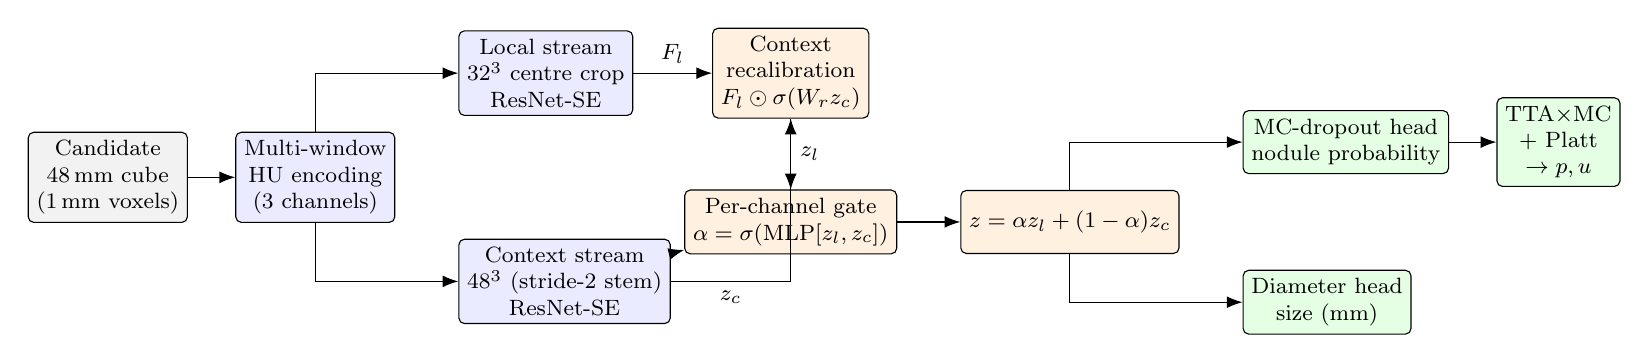
\begin{tikzpicture}[font=\footnotesize, node distance=4mm and 6mm,
  box/.style={draw, rounded corners=2pt, align=center, minimum height=8mm, inner sep=3pt},
  ar/.style={-{Latex[length=2mm]}}]
\node[box, fill=gray!10] (in) {Candidate\\48\,mm cube\\(1\,mm voxels)};
\node[box, right=of in, fill=blue!8] (mw) {Multi-window\\HU encoding\\(3 channels)};
\node[box, above right=2mm and 8mm of mw, fill=blue!8] (loc) {Local stream\\32$^3$ centre crop\\ResNet-SE};
\node[box, below right=2mm and 8mm of mw, fill=blue!8] (ctx) {Context stream\\48$^3$ (stride-2 stem)\\ResNet-SE};
\node[box, right=10mm of loc, fill=orange!12] (rec) {Context\\recalibration\\$F_l\odot\sigma(W_r z_c)$};
\node[box, below=9mm of rec, fill=orange!12] (gate) {Per-channel gate\\$\alpha=\sigma(\mathrm{MLP}[z_l,z_c])$};
\node[box, right=8mm of gate, fill=orange!12] (fuse) {$z=\alpha z_l+(1-\alpha)z_c$};
\node[box, above right=2mm and 8mm of fuse, fill=green!10] (cls) {MC-dropout head\\nodule probability};
\node[box, below right=2mm and 8mm of fuse, fill=green!10] (dia) {Diameter head\\size (mm)};
\node[box, right=6mm of cls, fill=green!10] (cal) {TTA$\times$MC\\+ Platt\\$\to p, u$};
\draw[ar] (in) -- (mw); \draw[ar] (mw) |- (loc); \draw[ar] (mw) |- (ctx);
\draw[ar] (loc) -- node[above]{$F_l$} (rec); \draw[ar] (ctx) -| node[pos=0.25,below]{$z_c$} (rec);
\draw[ar] (rec) -- node[right]{$z_l$} (gate); \draw[ar] (ctx) -- (gate);
\draw[ar] (gate) -- (fuse); \draw[ar] (fuse) |- (cls); \draw[ar] (fuse) |- (dia); \draw[ar] (cls) -- (cal);
\end{tikzpicture}}
\caption{MSGF-Net. Two 3D residual squeeze-excitation streams analyse a 32\,mm local and a 48\,mm context view; scale-gated fusion (orange) recalibrates local features with the context descriptor and mixes the scales with a learned gate. A classification head (sampled with MC dropout over 8 flipped views and calibrated) and a diameter head share the fused descriptor.}
\label{fig:arch}
\end{figure*}

\subsection{Multi-window encoding}
Each HU cube is mapped to three channels by clipping and scaling to $[0,1]$ with a lung window ($[-1350, 150]$\,HU), a mediastinal window ($[-160, 240]$) and a wide window ($[-1000, 400]$), exposing parenchymal texture and solid-tissue contrast simultaneously.

\subsection{Dual-scale encoder}
The local stream processes the central $32^3$ voxels and the context stream the full $48^3$ cube (stride-2 stem). Each stream is a 3D ResNet~\cite{he2016resnet} with six residual blocks with squeeze-excitation~\cite{hu2018se} (widths 24--48--96--96), producing feature maps $F_l$ and $F_c$ and global descriptors $z_c=\mathrm{GAP}(F_c)$.

\subsection{Scale-gated fusion}
The context descriptor first recalibrates the local channels, $F_l' = F_l\odot\sigma(W_r z_c)$, so that the surrounding anatomy can suppress, for example, round-blob evidence produced by a vessel crossing. With $z_l=\mathrm{GAP}(F_l')$, a per-channel gate decides how much each scale contributes:
\begin{equation}
\alpha=\sigma\big(\mathrm{MLP}([z_l; z_c])\big),\qquad z=\alpha\odot z_l+(1-\alpha)\odot z_c .
\end{equation}

\subsection{Heads and multi-task loss}
A classification head (dropout 0.3, FC-64, dropout, FC-1) and a diameter head ($\hat d=\mathrm{softplus}(w^\top z)+1$\,mm) share $z$. The loss combines the focal loss~\cite{lin2017focal} ($\gamma=2$, $\alpha=0.5$) with a smooth-L1 loss on log-diameter for positive candidates matched to a reference nodule, weighted by learned homoscedastic uncertainties~\cite{kendall2018multitask}:
\begin{equation}
\mathcal{L}=e^{-s_1}\mathcal{L}_{\mathrm{focal}}+s_1+e^{-s_2}\mathcal{L}_{\mathrm{diam}}+s_2 .
\end{equation}

\subsection{Training}
AdamW (learning rate $10^{-3}$, weight decay $10^{-4}$), one warm-up epoch and cosine decay, batch size 64, 24{,}000 samples per epoch with 25\% positives (sampled with replacement), 30 epochs with early stopping on validation AUC (patience 8). Augmentation: random flips on three axes, 90$^\circ$ in-plane rotations, $\pm$3\,mm shifts and HU scale/offset jitter ($0.97$--$1.03$, $\pm$20\,HU). Training ran in FP32 on a single NVIDIA Quadro P4000 (8\,GB) at about 7.9\,min per epoch (about 4\,h); the best validation AUC (0.997) was reached at epoch 22.

\subsection{Uncertainty-aware, calibrated inference}
For each candidate the two encoders are evaluated once for each of $V=8$ flip combinations, and the dropout head is sampled $M=10$ times per view, so the 80 probability samples cost only 8 encoder passes. The prediction is the mean $\bar p$ and the uncertainty $u$ is the standard deviation of the samples. Because positives are oversampled during training, $\bar p$ is mis-calibrated; we fit Platt scaling $p=\sigma(a\,\mathrm{logit}(\bar p)+b)$ on all 74{,}488 validation candidates ($a=1.634$, $b=-2.898$). The mapping is monotonic and therefore changes neither CPM nor AUC.

\subsection{Hard-negative fine-tuning (negative result)}
We also tested a second training round: the round-1 model scored all candidates of the training subsets, the 20 negatives with highest score per scan (9{,}846 patches) were added, and the model was fine-tuned for 10 epochs (learning rate $3\times10^{-4}$). Model selection on the validation subset rejected this variant (Section~\ref{sec:results}).

% =====================================================================================
\section{Evaluation}
\textbf{Detection:} FROC and CPM following~\cite{setio2017luna16} (a candidate within the radius of a reference nodule is a TP; excluded findings are ignored), with 95\% confidence intervals from 1{,}000 bootstrap resamples of scans; differences between variants use a paired bootstrap over scans (2{,}000 resamples). \textbf{Classification:} candidate-level AUC and average precision. \textbf{Calibration:} expected calibration error (ECE, 15 bins). \textbf{Size:} mean absolute error (MAE) and Pearson $r$ between predicted and reference diameter for positive candidates. \textbf{Uncertainty:} AUROC of $u$ for detecting misclassified candidates at $p\ge0.5$. \textbf{Model selection} among round-1, round-2 and their ensemble uses validation CPM only.

% =====================================================================================
\section{Results}\label{sec:results}
\subsection{Model selection}
On the validation subset the round-1 model achieved the highest CPM (Table~\ref{tab:select}) and was selected; the hard-negative round significantly lowered validation CPM ($-$0.028, 95\% CI $-$0.067 to $-$0.001, $p=0.037$), mainly at low FP rates (0.754$\to$0.636 at 1/8 FP/scan). Test results of all variants are listed for transparency only.

\begin{table}[t]
\centering
\caption{Model selection (CPM, single-pass inference). Selection uses subset 8 only.}
\label{tab:select}
\begin{tabular}{@{}lcc@{}}
\toprule
Variant & Validation (s8) & Test (s9)\\
\midrule
Round 1 (selected) & \textbf{0.861} & 0.882\\
Round 2 (hard negatives) & 0.833 & 0.888\\
Ensemble of round 1 + 2 & 0.852 & --\\
\bottomrule
\end{tabular}
\end{table}

\subsection{Detection performance}
Table~\ref{tab:main} reports the final model on the test subset. With uncertainty-aware inference MSGF-Net reaches CPM 0.903 (95\% CI 0.843--0.956), at the level of the best FP-reduction system in the LUNA16 challenge paper; TTA+MC raised CPM over single-pass inference by +0.019 on validation (95\% CI +0.001 to +0.040, paired bootstrap $p=0.040$) and by +0.022 on test ($-$0.006 to +0.039, $p=0.18$). Comparisons with the challenge results are indicative only: those systems were evaluated by 10-fold cross-validation on the earlier candidate set, whereas we report a single held-out fold with \texttt{candidates\_V2}. Fig.~\ref{fig:curves}a shows the FROC curve.

\begin{table*}[t]
\centering
\caption{Sensitivity at seven FP rates and CPM. Top: our model on the LUNA16 test subset (subset 9, 88 scans, 105 nodules). Bottom: FP-reduction systems reported in the LUNA16 challenge paper~\cite{setio2017luna16} (10-fold cross-validation on the original candidate set).}
\label{tab:main}
\small
\begin{tabular}{@{}lcccccccc@{}}
\toprule
Method & 1/8 & 1/4 & 1/2 & 1 & 2 & 4 & 8 & CPM (95\% CI)\\
\midrule
MSGF-Net, single pass & 0.714 & 0.810 & 0.876 & 0.905 & 0.924 & 0.962 & 0.981 & 0.882 (0.824--0.942)\\
MSGF-Net, TTA+MC+calibration (final) & \textbf{0.771} & \textbf{0.848} & \textbf{0.905} & 0.905 & 0.943 & 0.971 & 0.981 & \textbf{0.903} (0.843--0.956)\\
\midrule
CUMedVis~\cite{dou2017multilevel} & 0.677 & 0.834 & 0.927 & 0.972 & 0.981 & 0.983 & 0.983 & 0.908\\
JackFPR & 0.734 & 0.796 & 0.859 & 0.892 & 0.923 & 0.944 & 0.954 & 0.872\\
DIAG\_CONVNET & 0.669 & 0.760 & 0.831 & 0.892 & 0.923 & 0.945 & 0.960 & 0.854\\
ZNET & 0.511 & 0.630 & 0.720 & 0.793 & 0.850 & 0.884 & 0.915 & 0.758\\
\bottomrule
\end{tabular}
\end{table*}

\subsection{Comparison with standard architectures}
To separate the contribution of the network from that of the training and inference protocol, we trained three widely used architectures with exactly the same split, sampling, multi-window input, augmentation, focal and diameter losses, training budget with early stopping on validation AUC, and inference (8-view TTA with MC dropout); only the network differs, and each uses the 32\,mm local view with the same classification and diameter heads. The baselines are a 3D ResNet-18~\cite{he2016resnet} with the standard stride-2 stem and max-pooling (33.2\,M parameters), a 2.5D ResNet-18 that receives the axial, coronal and sagittal centre planes of the three HU windows as nine input channels (11.2\,M), and a plain 3D CNN of four double-convolution blocks with max-pooling, the classic FP-reduction design (3.5\,M). Table~\ref{tab:arch} shows the results. MSGF-Net outperforms the 3D ResNet-18 (+0.048 CPM, 95\% CI +0.003 to +0.088, $p=0.034$) with one tenth of its parameters and is ahead of the 2.5D ResNet-18 without a significant difference (+0.042, $p=0.14$). The plain 3D CNN, however, matches MSGF-Net ($-$0.004, $p=0.68$). We therefore do not claim that the architecture alone improves detection: at this test size most of the accuracy is attributable to the shared protocol (multi-window encoding, hard-negative-aware sampling, TTA and MC dropout). MSGF-Net retains the lowest uncalibrated ECE and size error, provides the interpretable scale gate and the context stream used for large nodules, and is cheaper to run: because the plain CNN convolves its first two blocks at full resolution, it needed about three times longer per training epoch (${\approx}$1{,}470\,s vs.\ ${\approx}$470\,s) and 2.3 times longer to score the test subset (134 vs.\ 58\,min).

\begin{table*}[t]
\centering
\caption{Standard architectures trained and evaluated with the identical protocol (LUNA16 test subset 9, TTA+MC, no calibration). $\Delta$CPM = MSGF-Net minus baseline, paired scan-level bootstrap.}
\label{tab:arch}
\small\setlength{\tabcolsep}{4.5pt}
\begin{tabular}{@{}lcccccc@{}}
\toprule
Network & Params & CPM (95\% CI) & Sens.\ @1 / @4 FP & ECE & Size MAE & $\Delta$CPM (95\% CI), p\\
\midrule
\textbf{MSGF-Net (ours)} & 3.35\,M & 0.903 (0.843--0.956) & 0.905 / 0.971 & \textbf{0.012} & \textbf{0.45\,mm} & --\\
Plain 3D CNN & 3.53\,M & 0.908 (0.857--0.953) & 0.943 / 0.971 & 0.015 & 0.49\,mm & $-$0.004 ($-$0.031, +0.021), 0.68\\
2.5D ResNet-18 & 11.21\,M & 0.861 (0.812--0.923) & 0.876 / 0.933 & 0.122 & 0.67\,mm & +0.042 ($-$0.010, +0.085), 0.14\\
3D ResNet-18 & 33.24\,M & 0.856 (0.796--0.917) & 0.857 / 0.943 & 0.061 & 0.93\,mm & +0.048 (+0.003, +0.088), 0.034\\
\bottomrule
\end{tabular}
\end{table*}

\subsection{Clinical outputs: size, calibration, uncertainty}
On the test subset the diameter head estimates nodule size with an MAE of 0.45\,mm ($r=0.996$), so the size-based Lung-RADS category can be proposed automatically. Platt scaling fitted on the validation subset reduces the test ECE from 0.0123 to 0.0007 (Fig.~\ref{fig:curves}b). The predictive uncertainty separates wrong from correct decisions with an AUROC of 0.971: all 89 errors of the model (at $p=0.5$) lie among the 5\% most uncertain candidates (about 43 per scan), so referring this group to the radiologist would catch every error, whereas referring the same number at random would catch about 5\% of them (Fig.~\ref{fig:curves}c). The very top of the ranking is less selective (2\% referred catches 17\% of errors), because uncertainty is also high for borderline candidates that the model classifies correctly. The fusion gate is interpretable: the mean weight on the local stream increases with nodule size (Spearman $\rho=0.77$ on positive test candidates).

\begin{figure*}[t]
\centering
\begin{tabular}{ccc}
\figorbox{figures/froc.png}{0.31\textwidth} & \figorbox{figures/reliability.png}{0.25\textwidth} & \figorbox{figures/triage.png}{0.31\textwidth}\\
(a) FROC, test subset & (b) reliability after calibration & (c) uncertainty-based triage
\end{tabular}
\caption{Final model on the LUNA16 test subset.}
\label{fig:curves}
\end{figure*}

\subsection{Ablation study}
Table~\ref{tab:ablation} removes one component at a time (10 epochs, single-pass inference, same split and seed). No ablation changed CPM significantly (paired bootstrap, all $p\ge0.25$; differences within $\pm$0.02), and the reference model trained for 10 epochs (0.908) scored higher than the 30-epoch model with the same single-pass inference (0.882; $\Delta$ +0.026, $p=0.25$), indicating that differences of this size are within run-to-run variation. Removing the diameter task did not reduce CPM but eliminated size estimation (MAE 9.9\,mm). We therefore do not claim that individual components improve detection accuracy; the evidence supports that the additional clinical outputs are obtained without a measurable loss of detection performance. Ablation results were not used for model selection.

\begin{table}[t]
\centering
\caption{Ablations on the test subset (10 epochs, single pass). $\Delta$ vs.\ full model; p from paired bootstrap.}
\label{tab:ablation}
\small
\begin{tabular}{@{}lccc@{}}
\toprule
Variant & CPM & $\Delta$ & p\\
\midrule
Full MSGF-Net & 0.908 & -- & --\\
w/o context stream & 0.909 & +0.001 & 0.95\\
Concat instead of SGF & 0.898 & $-$0.010 & 0.62\\
Single HU window & 0.903 & $-$0.004 & 0.74\\
w/o diameter task$^\dagger$ & 0.924 & +0.016 & 0.44\\
BCE instead of focal loss & 0.925 & +0.018 & 0.25\\
\bottomrule
\multicolumn{4}{@{}l}{\footnotesize $^\dagger$no size output (diameter MAE 9.9 mm vs.\ 0.80 mm).}
\end{tabular}
\end{table}

% =====================================================================================
\section{External Validation on LUNA25}
\textbf{Data.} LUNA25~\cite{luna25} contains 4{,}069 low-dose screening CTs of the National Lung Screening Trial~\cite{nlst2011} with 6{,}163 annotated nodules (555 malignant) from 2{,}120 patients, acquired with different scanners and protocols than LIDC-IDRI. It provides nodule locations but no non-nodule candidates, so FPs per scan cannot be counted; we therefore measure nodule-level sensitivity at fixed operating points: the probability thresholds that produced 1/8 \dots\ 8 FPs per scan on the LUNA16 \emph{validation} subset, chosen before any LUNA25 data were seen. The same thresholds are applied to the LUNA16 test subset for comparison. The model is applied unchanged (no fine-tuning); 95\% CIs come from a patient-level bootstrap.

\begin{table}[t]
\centering
\caption{External validation without retraining: sensitivity at operating points fixed on LUNA16 validation.}
\label{tab:luna25}
\small
\resizebox{\columnwidth}{!}{\begin{tabular}{lcccc}
\toprule
FP/scan & LUNA16 & \multicolumn{3}{c}{LUNA25 (6{,}163 nodules)} \\
(LUNA16 val) & test & all (95\% CI) & malignant & benign \\
\midrule
1/8 & 0.838 & 0.589 (0.571--0.606) & 0.636 & 0.584 \\
1/4 & 0.867 & 0.629 (0.612--0.646) & 0.661 & 0.626 \\
1/2 & 0.905 & 0.688 (0.672--0.704) & 0.699 & 0.687 \\
1   & 0.914 & 0.756 (0.741--0.771) & 0.759 & 0.756 \\
2   & 0.971 & 0.831 (0.818--0.843) & 0.811 & 0.833 \\
4   & 0.971 & 0.876 (0.865--0.887) & 0.847 & 0.879 \\
8   & 0.981 & 0.907 (0.897--0.916) & 0.872 & 0.910 \\
\midrule
mean & 0.921 & 0.754 & & \\
\bottomrule
\end{tabular}}
\end{table}

Table~\ref{tab:luna25} shows a clear but expected domain shift: mean sensitivity falls from 0.921 to 0.754, while at 8 FPs per scan on LUNA16 terms the model still finds 90.7\% of LUNA25 nodules. Two factors are likely: LUNA25 is low-dose screening CT with a higher noise level, and its annotations include many small and subsolid nodules that LUNA16's consensus criterion ($\ge$3\,mm, accepted by 3 of 4 readers) excludes. Malignant nodules are detected at least as well as benign ones at strict operating points. Because LUNA25 has malignancy labels, it also supports a cancer-risk model built on the same architecture; that work is reported separately.

\section{Privacy-Preserving Federated Training}\label{sec:fed}
Hospitals rarely may pool CT data. We therefore simulated four hospitals that never exchange images: the LUNA16 training subsets were split by subset (patient-disjoint) into sites A (subsets 0--1), B (2--3), C (4--5) and D (6--7), each holding about 6{,}600 training patches. With federated averaging (FedAvg)~\cite{mcmahan2017fedavg}, every round each site starts from the global model, trains on 6{,}000 of its own patches and returns only its weights, which the server averages (weighted by site size, including batch-normalisation statistics); 20 rounds were run. Compute was matched: one round equals one central epoch of 24{,}000 patches, and the same 20 epochs were used for a model trained on all data pooled (the privacy-violating upper bound) and for a model trained by site A alone (what a single hospital could do). All three were selected on validation AUC (subset~8) and tested on subset~9 with single-pass inference and no calibration, so absolute values are below Table~\ref{tab:main}.

\begin{table}[t]
\centering
\caption{Federated training across four simulated hospitals (test subset 9, single-pass inference). $p$: paired patient-level bootstrap vs FedAvg.}
\label{tab:fed}
\setlength{\tabcolsep}{4pt}
\resizebox{\columnwidth}{!}{%
\begin{tabular}{lcccc}
\toprule
Training data & Val AUC & Test CPM (95\% CI) & Sens.\ @1 FP & $p$ \\
\midrule
Hospital A alone & 0.984 & 0.665 (0.583--0.744) & 0.657 & $<0.001$ \\
FedAvg, 4 hospitals (weights only) & 0.994 & 0.808 (0.740--0.883) & 0.810 & -- \\
All data pooled (upper bound) & 0.997 & 0.880 (0.819--0.935) & 0.914 & 0.002 \\
\bottomrule
\end{tabular}}
\end{table}

Table~\ref{tab:fed} shows that collaboration without sharing data is clearly worthwhile: FedAvg raises CPM by $+0.143$ (95\% CI $+0.101$ to $+0.196$) over a single hospital and closes about two thirds of the gap to pooled training, which remains better by $0.072$ ($+0.023$ to $+0.121$). The validation AUC hides most of these differences (0.984--0.997); the FROC-based CPM on whole scans reveals them. Our sites are drawn from one dataset and are therefore more similar than real hospitals, so the federated result is likely optimistic; each round exchanges about 107\,MB of weights.

\section{End-to-End System}
\subsection{Candidate finder for new scans}
A deployed system cannot use \texttt{candidates\_V2}. Our training-free finder resamples the scan to 1\,mm, builds a lung mask, computes a multi-scale scale-normalised Laplacian-of-Gaussian (LoG) blob response ($\sigma = 1.5$--8\,mm) and keeps local maxima inside the mask with HU $> -700$. Developing it on the held-out subset exposed two failure modes. First, many scans have a circular reconstruction field of view whose padding, after resampling, forms a rim of air-like values that connects the lungs to the outside air; a mask built from air components then fails (on about 25 of 88 scans). We remove the dilated padding before labelling, select lung components by size and by mean density (lungs contain vessels; pure air is about $-1000$\,HU), fall back to a slice-wise ``air enclosed by the body'' criterion, and close the mask with a 10\,mm disk so that juxtapleural nodules stay inside. Second, ranking peaks by LoG response alone lets bright vessel segments crowd out small nodules. We therefore rank candidates by LoG response times a Hessian blobness score $\lambda_3/\lambda_1 \in [0,1]$ (computed only at the peaks, at their own scale), which is near 1 for spheres and near 0 for tubes and plates, reserve 150 places for large blobs ($\sigma \ge 4$\,mm) and keep 1{,}000 candidates per scan.

\begin{table}[t]
\centering
\caption{Complete pipeline on LUNA16 test subset~9 (88 scans, 105 nodules): candidate recall by nodule diameter and end-to-end CPM.}
\label{tab:e2e}
\small
\setlength{\tabcolsep}{3.5pt}
\resizebox{\columnwidth}{!}{\begin{tabular}{lccccccc}
\toprule
Finder & 3--6 & 6--10 & 10--20 & $\ge$20 & recall & CPM (95\% CI) \\
\midrule
v2: air-component mask & 18/45 & 16/34 & 16/20 & 6/6 & 0.533 & 0.529 (0.42--0.66) \\
v3: + padding fix, 1{,}000 cand. & 30/45 & 21/34 & 17/20 & 6/6 & 0.705 & 0.683 (0.55--0.82) \\
v4: + body fallback & 34/45 & 22/34 & 17/20 & 6/6 & 0.752 & 0.721 (0.59--0.85) \\
\textbf{v5: + blobness ranking} & \textbf{40/45} & \textbf{31/34} & \textbf{20/20} & \textbf{6/6} & \textbf{0.924} & \textbf{0.867 (0.80--0.92)} \\
\midrule
\texttt{candidates\_V2} (reference) & & & & & & 0.903 (0.84--0.96) \\
\bottomrule
\end{tabular}}
\end{table}

Table~\ref{tab:e2e} shows that the classifier is not the bottleneck: of the nodules that reach it, MSGF-Net finds most at 1/8 FP per scan. With finder v5, the complete system scores CPM 0.867 with sensitivities of 0.771, 0.876 and 0.924 at 1/8, 1 and 8 FPs per scan, close to the 0.903 obtained with the challenge candidates. All nodules of 10\,mm or more are reached. \textbf{Runtime.} For the workstation, the finder's filters run on the GPU (same kernels and border handling as the CPU version; identical candidates up to floating-point ties) and classification is done in two stages: one plain pass over all candidates, then full TTA and MC dropout only for the 150 highest-scoring candidates and any with probability $\ge 0.05$. On the same 88 test scans this lowers the analysis time from about 4.5\,min to 72\,s per scan on the Quadro P4000, with CPM 0.864 (95\% CI 0.795--0.923) versus 0.867 for full scoring of every candidate.

\subsection{Clinician workstation and patient application}
Both applications are written in Flutter and communicate over a token-authenticated REST API with a Python server that runs the models on the GPU workstation. The \emph{clinician workstation} (Flutter app for the browser, Windows and Android tablets, with role-based login and an audit log) accepts MetaImage, NIfTI or DICOM studies and shows each suspected nodule on a slice viewer with its calibrated probability, uncertainty flag, estimated size and size-based Lung-RADS category (Fig.~\ref{fig:apps}). A slice-level risk bar colours every slice green, yellow or red (default thresholds 30\% and 70\%, set by the administrator), and a Grad-CAM~\cite{selvaraju2017gradcam} overlay computed on the local stream shows the image region that drove each decision. Two cancer-risk estimates are displayed side by side and not merged: an image-based estimate from a separate LUNA25-trained model and the published Brock (PanCan) clinical model~\cite{mcwilliams2013brock}, which uses the patient's age, sex, family history and emphysema together with nodule size, type, location, count and spiculation. The radiologist confirms or rejects each finding, writes an impression and releases the study. Only then does the \emph{patient application} (Flutter, Android) show it, without rejected findings. Its assistant is a tool-using agent that reads the released results, derives the follow-up date from the radiologist's instruction or, if absent, from size-based Lung-RADS guidance, sets reminders, keeps a symptom diary with red-flag escalation, messages the clinic and answers general questions only from a retrieval index of approved guideline summaries (Lung-RADS, WHO, USPSTF), citing the source. It never diagnoses or quantifies cancer risk for the patient, and runs either with a large language model or with an offline rule-based planner.

\begin{figure*}[t]
\centering
\figorbox{figures/app_doctor.png}{0.56\textwidth}\hfill
\figorbox{figures/app_patient_home.png}{0.2\textwidth}\hfill
\figorbox{figures/app_patient_chat.png}{0.21\textwidth}
\caption{Left: Flutter clinician workstation on a LUNA16 test scan: a 23.9\,mm nodule (nodule probability 90.0\%) with the Grad-CAM overlay switched on, the slice-level risk bar (green/yellow/red) below the image, and side-by-side image-based AI cancer risk (53.2\%) and Brock clinical risk (6.4\%; computed from the patient's data and the nodule features set by the doctor). Middle and right: the patient application after the radiologist released the study, showing the plain-language summary, follow-up date and an urgent red-flag escalation in the assistant.}
\label{fig:apps}
\end{figure*}

\section{Discussion and Limitations}
MSGF-Net reaches detection performance comparable to the best LUNA16 FP-reduction systems with a single compact network, and adds outputs that matter for clinical use: nodule size, calibrated probabilities and a reliable uncertainty signal. Several limitations apply. (i) We report one held-out fold rather than the full 10-fold protocol, and the test subset contains 105 nodules, hence the wide confidence intervals. (ii) Ablations and the architecture comparison used a single seed; a plain 3D CNN trained with our protocol matched MSGF-Net, so the architectural contribution to detection accuracy is not established. (iii) LUNA16 contains no malignancy labels; the detector does not estimate cancer risk, and the risk estimates shown in the workstation come from separate models. (iv) Lung-RADS categories are derived from size alone, without nodule type or growth. (v) The candidate finder was developed while looking at subset~9 (its design choices v2--v5 were driven by the failures observed there), so its end-to-end CPM is optimistic and should be confirmed on other subsets or on LUNA25. (vi) The external LUNA25 test measures sensitivity only, because the dataset has no non-nodule candidates. (vii) The federated experiment simulates hospitals by splitting one dataset, a single run per setting. (viii) The applications are research prototypes and have not been evaluated with radiologists or patients.

\section{Conclusion}
We presented a calibrated, uncertainty-aware 3D FP-reduction network with scale-gated fusion and size estimation that achieves CPM 0.903 on a held-out LUNA16 subset, outperforms a much larger 3D ResNet-18 under an identical protocol, provides sub-millimetre size estimates and well-calibrated, self-aware probabilities, and is deployed in clinician and patient applications. Behind a robust, blobness-ranked candidate finder the complete system reaches CPM 0.867 from raw CT, and it transfers to independent screening data with a measurable but moderate loss in sensitivity. Trained by federated averaging across four simulated hospitals that share only model weights, it recovers about two thirds of the benefit of pooling their data. Code: \url{https://github.com/mabdullah52/FYP-Project}.

\IfFileExists{IEEEtran.bst}{\bibliographystyle{IEEEtran}}{\bibliographystyle{unsrt}}
\bibliography{refs}

\end{document}
